\begin{figure}[htp]
\caption{Medien \& Mediennutzung}\label{fig:AppMediennutzung}
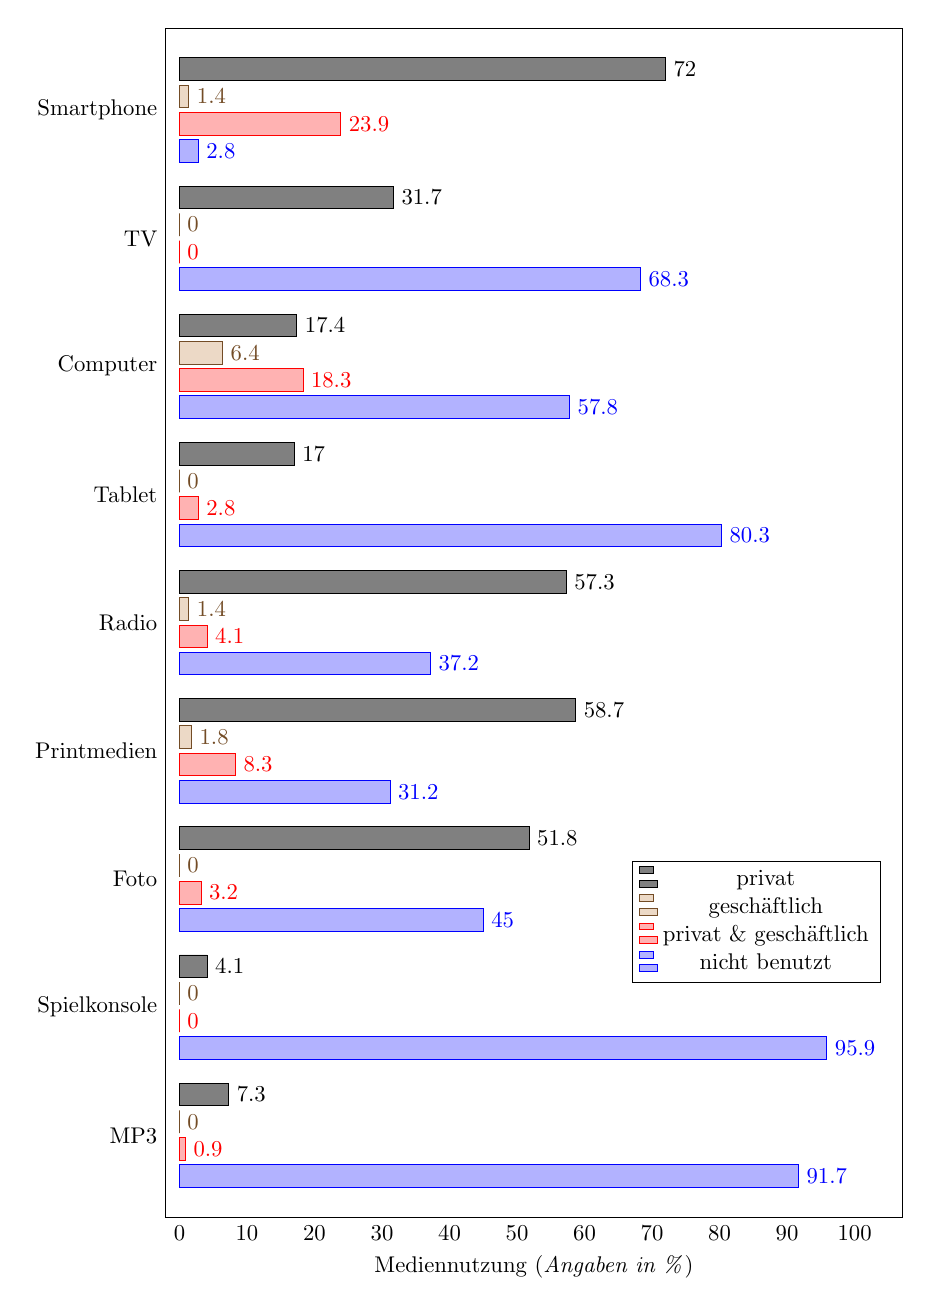
\begin{tikzpicture}[scale=0.82, auto]
  \begin{axis}[
    xbar,
    %y axis line style = { opacity = 0 },
    %axis x line       = none,
    tickwidth         = 0pt,
    xmin              = 0,
    xmax              = 105,
    enlarge y limits  = 0.08,
    enlarge x limits  = 0.02,
    reverse legend,
    %/legend pos=south east,
    legend style={at={(0.97,0.3)}},
    ytick             = data,
    xlabel            = {Mediennutzung (\textit{Angaben in \%})},
    height            = 20cm,
    width             = 13cm,
    symbolic y coords = {MP3, Spielkonsole, Foto, Printmedien, Radio, Tablet, Computer, TV, Smartphone},
    nodes near coords,
    nodes near coords align={horizontal},
  ]
  %nicht benutzt
  \addplot coordinates { (2.8,Smartphone)(68.3,TV)(57.8,Computer)(80.3,Tablet)(37.2,Radio)(31.2,Printmedien)(45,Foto)(95.9,Spielkonsole)(91.7,MP3)};
  %privat und geschäftlich
  \addplot coordinates { (23.9,Smartphone)(0,TV)(18.3,Computer)(2.8,Tablet)(4.1,Radio)(8.3,Printmedien)(3.2,Foto)(0,Spielkonsole)(0.9,MP3)};
  %geschäftlich
  \addplot coordinates { (1.4,Smartphone)(0,TV)(6.4,Computer)(0,Tablet)(1.4,Radio)(1.8,Printmedien)(0,Foto)(0,Spielkonsole)(0,MP3)};
  %privat
  \addplot coordinates { (72,Smartphone)(31.7,TV)(17.4,Computer)(17,Tablet)(57.3,Radio)(58.7,Printmedien)(51.8,Foto)(4.1,Spielkonsole)(7.3,MP3)};
  
  \legend{nicht benutzt, privat \& geschäftlich, geschäftlich, privat}
  \end{axis}
\end{tikzpicture}
\end{figure}
